\documentclass[a4paper, 12pt]{report}

\usepackage{longtable}
\usepackage{lipsum}					% Als Platzhalter f�r gewisse Stellen
\usepackage{ngerman}					%Deutsche Silbentrennung etc.
\usepackage[latin1]{inputenc}	% Umlaute in .tex Files normal schreibbar
% Unter texnic-center alle Quelldateien unter Codierung ANSI abspeichern
% Auf Unixsystemen ISO 8859-15
\usepackage{helvet}						%Helvetic als Schriftart
\usepackage{courier}					%Courier als Schriftart f�r Listings
\usepackage{fancyhdr}					%Kopf- und Fu�zeilen �ndern
\usepackage{a4}								%A4 Randeinstellungen
\usepackage{makeidx}					%Indexkommandos
\usepackage{listings}					%F�r zeilennummerierte Listings mit Hintergrund
\usepackage{color}					%F�r grauen Hintergrund in Listings
\usepackage{setspace}					%Gr��erer Zeilenabstand
\usepackage{graphicx}					%Grafiken einbinden
\usepackage{sectsty}					%Format der �berschriften um�ndern
\usepackage{hyperref}
\usepackage{float}
\usepackage{pdfpages}					%Fremde pdfs einbinden
\usepackage[font={scriptsize}]{caption}


%Dokumentationen zu den Paketen finden sich im Installationsordner 
%(normalerweise C:\Programme\texmf) unter docs und dort auch im Unterverzeichnis latex.

%Das Kompilieren des Dokuments ben�tigt bis zu 3 Durchl�ufe im alle Referenzen und
%Literatureintr�ge korrekt einzubinden.

%----------------------------------------------------------------------------------
% Listings 
%----------------------------------------------------------------------------------

%Definition des Aussehens der externen Listings
\def\source#1#2#3{     %  Sprache, Caption, Dateiname 
  %\global\advance\Sourcenummer by 1 
  %\index{Listing #1 #2}
  %\textbf{Listing-\the\Sourcenummer: #2}
  \lstinputlisting[language=#1,caption=#2]{#3} 
}

% Beispiele f�r eine Verwendung
%--------------------------------------------------------------------------------
% \source{xml}{\texttt{faces-config.xml}}{sources/faces-config.xml}
%
% \source{java}{\texttt{beans.UserBean.java}}{sources/jsf/user/UserBean.java}
%---------------------------------------------------------------------------------


%Definition des Aussehens der internen Listings
\definecolor{listinggray}{gray}{1.0}

%-------------------------------------------------------------------------
% Neues Listingformat
% --- kleine Schrift
% --- Keywords f�rbig
%-------------------------------------------------------------------------

\definecolor{dkgreen}{rgb}{0,0.6,0}
\definecolor{gray}{rgb}{0.5,0.5,0.5}
\definecolor{mauve}{rgb}{0.58,0,0.82}
\definecolor{orange}{RGB}{240, 105, 12}

\lstset{ %
  language=Java,                  % the language of the code
  basicstyle=\footnotesize\ttfamily\bfseries,       % the size of the fonts that are used for the code
  numbers=left,                   % where to put the line-numbers
  numberstyle=\footnozesize,      % the size of the fonts that are used for the line-numbers
  stepnumber=1,                   % the step between two line-numbers. If it's 1, each line 
                                  % will be numbered
  numbersep=5pt,                  % how far the line-numbers are from the code
  backgroundcolor=\color{white},  % choose the background color. You must add \usepackage{color}
  showspaces=false,               % show spaces adding particular underscores
  showstringspaces=false,         % underline spaces within strings
  showtabs=false,                 % show tabs within strings adding particular underscores
  frame=single,                   % adds a frame around the code
  tabsize=2,                      % sets default tabsize to 2 spaces
  captionpos=b,                   % sets the caption-position to bottom
  breaklines=true,                % sets automatic line breaking
  breakatwhitespace=false,        % sets if automatic breaks should only happen at whitespace
  title=\lstname,                 % show the filename of files included with \lstinputlisting;
                                  % also try caption instead of title
  numberstyle=\tiny\color{gray},  % line number style
  keywordstyle=\color{blue},      % keyword style
  commentstyle=\color{dkgreen},   % comment style
  stringstyle=\color{mauve},      % string literal style
  escapeinside={\%*}{*)},         % if you want to add a comment within your code
  morekeywords={*,...}            % if you want to add more keywords to the set
}

%-------------------------------------------------------------------------
% Listings aus der ersten Version: Grosse Schrift, Schwartz-weiss
%-------------------------------------------------------------------------


% \lstset{
% 	language=Java,
% 	frame=ltrb
% 	backgroundcolor=\color{listinggray},
% 	%basicstyle=\linespread{1.0}\ttfamily\small,
% 	basicstyle=\linespread{1.0}\ttfamily\small,
% 	commentstyle=\textit,
% 	tabsize=2,
% 	float=ph,
% 	extendedchars,
% 	breaklines,
% 	prebreak={\space\hbox{\ensuremath\hookleftarrow}},,
% 	numbers=left,
% 	numberstyle=\small,
% 	stringstyle=\textsl,
% 	showstringspaces=false,
% 	captionpos=b,
% 	aboveskip=16pt
% }


%Eigene Kommandos
\newcommand{\zb}{z.B.\ }				%z.B.
\newcommand{\tm}{\texttrademark \ }			%TM - Zeichen
\newcommand{\sk}[1]{\emph{siehe Kapitel \ref{#1}}}	%siehe Kapitel <Referenz>
\newcommand{\lil}[1]{\emph{Listing \ref{#1}}}		%Listing <Referenz>
\newcommand{\slil}[1]{\emph{siehe Listing \ref{#1}}}	%siehe Listing <Referenz>
\newcommand{\pr}{$\rightarrow\ $}			%Pfeil nach rechts


%-------------------------------------------------------------------------------
% Uebersichten i Anhang richtig formatieren
%-------------------------------------------------------------------------------

\makeatletter
\renewcommand*\l@section{\@dottedtocline{2}{3.8em}{4em}}
\renewcommand*\l@subsection{\@dottedtocline{2}{3.8em}{4em}}
\renewcommand*\l@subsubsection{\@dottedtocline{2}{3.8em}{4em}}
\renewcommand*\l@figure{\@dottedtocline{1}{2.8em}{3em}}
\renewcommand*\l@lstlisting{\@dottedtocline{1}{2.8em}{3em}}
\makeatother

%Es soll ein Index f�r diese Diplomarbeit erzeugt werden
%\makeindex

%L�ngen- und Absatzeinstellungen
\parindent=0pt		%Kein Einr�cken der ersten Zeile eines Absatzes
\parskip=12pt			%12pt Abstand zwischen 2 Abs�tzen
%\doublespacing 	 %Doppelter Zeilenabstand
\onehalfspacing	  %Eineinhalbfacher Zeilenabstand

\setlength{\headheight}{15pt}		%Kopfzeile vergr��ern (wegen 12pt Schriftgr��e)	
\addtolength{\textwidth}{1.5cm}	%Rechten Rand verkleinern


%--------------------------------------------------------------------------
% Beginn Dokument
%--------------------------------------------------------------------------


\begin{document}
	\sffamily											%Schriftart setzen
	\allsectionsfont{\sffamily}		%Schrift f�r �berschrift setzen
	
	\pagestyle{empty}
\singlespacing
\sffamily

\begin{flushleft}
	
\includegraphics[scale=0.20]{images/HTL_IF.png} \\
% 	\vspace{-2cm}
% 	\hspace{7cm}
% 	\Huge
% 	\textbf{- Diplomarbeit -} \\
% 	\hrulefill
\end{flushleft}
\vspace{-3cm}
\begin{flushright}
	
\includegraphics[scale=0.10]{images/HTL.jpg} \\
% 	\vspace{-2cm}
% 	\hspace{7cm}
% 	\Huge
% 	\textbf{- Diplomarbeit -} \\
% 	\hrulefill
\end{flushright}

\vspace{-2.5cm}
\begin{center}
\textbf{HTBLuVA St. P�lten}\\
\textbf{H�here Abteilung f�r Informatik}
\end{center}
\vspace{-0.5cm}
\hrulefill

\begin{center}
\vspace{2cm}
\huge
\textbf{DIPLOMARBEIT}

\huge
\textbf{Einsatz von Java FX}

\large
\textbf{im Projekt Eventtechnik}
\end{center}

\begin{flushleft}
\large
\vspace{3cm}
\begin{small}
\begin{tabular}{lp{2cm}l}

\textbf{Ausgef�hrt im Schuljahr 2014/15 von:} &  & \textbf{Betreuer/Betreuerin:} \\
\\																
Simon Lehner-Dittenberger, 5AHIF-10 & & OSTR Mag. Otto Reichel \\
\end{tabular}
\end{small}
\end{flushleft}

\vspace{1cm}

St.P�lten, am \today									%Externe .tex Datei f�r Titel einbinden
	\clearpage										%Neue Seite beginnen

	
%-----------------------------------------------------------------
% Vorwort
%-----------------------------------------------------------------
	
	\pagestyle{plain}							%Nur Fu�zeile mit Seitennummer anzeigen lassen
	\pagenumbering{roman}					%R�mische Nummerierung vor der eigentlichen Diplomarbeit
	\setcounter{page}{1}					%Bei 1 mit Nummerierung beginnen

  \addcontentsline{toc}{chapter}{Vorwort}
	\addcontentsline{toc1}{section}{Erkl�rung}	%Erkl�rung h�ndisch ins Inhaltsverzeichnis einf�gen
	\begin{flushleft}
\Large
\textbf{Eidesstattliche Erkl�rung\\}
\vspace{1.5cm}
\end{flushleft}


Ich erkl�re an Eides statt, dass ich die vorliegende Diplomarbeit selbst�ndig und ohne fremde Hilfe verfasst, andere als die angegebenen Quellen
und Hilfsmittel nicht benutzt und die den benutzten Quellen w�rtlich und inhaltlich entnommenen Stellen als solche erkenntlich gemacht habe.

\begin{center}
	\vspace{1.5cm}
	\rule{200pt}{1pt} \\
	Simon Lehner-Dittenberger
	
\end{center}

St.P�lten, am 24.04.20XX
	
	
												%Externe .tex Datei f�r Erkl�rung einf�gen
	\newpage																  %Neue Seite beginnen
	\phantomsection
	
	\addcontentsline{toc}{section}{Diplomandenvorstellung}
	\begin{flushleft}
\Large
\textbf{Diplomandenvorstellung\\}
\vspace{1.5cm}
\end{flushleft}

\vspace{1cm}

\begin{flushleft}
% Hier ist ein Bild des Diplomanden%
\hspace{3cm} 
\includegraphics[scale=0.3]{images/HTL_IF.png} 

\vspace{-0.9cm}
\hspace{6cm}
\textcolor{orange}{\rule{8cm}{5pt}}
\end{flushleft}


\begin{tabular}{p{3cm}l}
& Max MUSTERMANN \\
\\
& Geburtsdaten: \\
&06.02.1996 in Musterort \\
\\
&Wohnhaft in: \\
&Musterstra�e 13/1 \\
&3100 Musterstadt \\
\\
&Werdegang:\\
&2010 - 2015: \\
&HTBLuVA St.P�lten, Abteilung f�r Informatik\\
&2006 - 2010: \\
&Bundesrealgymnasium Wieselburg a. d. Erlauf\\
\\
&Kontakt:\\
&max.mustermann@gmx.at\\
\end{tabular}
	\newpage
	\phantomsection
	
	\addcontentsline{toc}{section}{Danksagungen}
	\begin{flushleft}
	\Large
	\textbf{Danksagungen\\}
	\vspace{1.5cm}
	
	\large
	Danke
\end{flushleft}
	\newpage
	\phantomsection
	

	\addcontentsline{toc}{section}{Zusammenfassung}
	\begin{flushleft}
	\Large
	\textbf{Zusammenfassung\\}
	\vspace{1.5cm}
	
\end{flushleft}
	\newpage
	\phantomsection
	
	\addcontentsline{toc}{section}{Abstract}
	\begin{flushleft}
	\Large
	\textbf{Abstract\\}
	\vspace{1.5cm}
	
\end{flushleft}
	\newpage
	\phantomsection
	
	\normalsize

	\markright{INHALTSVERZEICHNIS}
	\addcontentsline{toc}{chapter}{Inhaltsverzeichnis}
	\tableofcontents
	\newpage
	\phantomsection
	
		
%-----------------------------------------------------------------
% Kopfzeilen definieren
%-----------------------------------------------------------------
	\pagestyle{fancyplain}

	\renewcommand{\sectionmark}[1]{\markright{\thesection\ #1}}
	\renewcommand{\chaptermark}[1]{\markright{\thechapter\ #1}}
	\lhead[\fancyplain{}{\sffamily\sl\thepage}]{\fancyplain{}{\sffamily\sl\rightmark}}
	\rhead[\fancyplain{}{\sffamily\sl\leftmark}]{\fancyplain{}{\sffamily\sl\thepage}}
	\cfoot{}

	\pagenumbering{arabic}	%Seiten wieder normal nummerieren
	\setcounter{page}{1}		%Bei 1 beginnen

%--------------------------------------------------------------------------
% Kapitel einf�gen
%--------------------------------------------------------------------------

	\newcommand{\todo}[1]{{\color{red} \footnote{\color{red} TODO #1}}}
	\newcommand{\doublehref}[1]{\href{#1}{#1}}
	\clearpage
	\chapter{�bersicht}

	\section{Was ist Steganographie}
	
	Die Steganographie ist eine Methode, die sich mit dem Verstecken von zu �bermittelnden Nachrichten besch�ftigt und kam schon in der Antike zum Einsatz. Das Wort kommt aus den griechischen W�rtern ''stegano'' und ''graphein'', was �bersetzt ''bedeckt schreiben'' bedeutet \cite{L: StegoGeschichte}. Dabei wird meist ein Text, aber auch andere Arten von Informationen, in einem Tr�germedium versteckt. Diese Kombination wird als Steganogramm bezeichnet. Das Medium sollte so gew�hlt sein, dass sich die einzubettenden Daten leicht integrieren lassen. Au�erdem ben�tigt es ein gewisses Ma� an Entropie, damit Unregelm��igkeiten nicht so stark auffallen, denn eine Blume ist in einer bunten Blumenwiese schwerer zu finden, als auf einem asphaltierten Parkplatz. Ziel ist es immer, die Wahrnehmungsschwelle eines Menschen so weit zu unterschreiten, dass man gar nicht auf die Idee kommt �berhaupt nach einer versteckten Nachricht zu suchen. 
	\todo{Welche Techniken wof�r gut sind und welche Tr�germaterialen man braucht wird in den sp�teren abschnitten behandelt}
	
	
	Die M�glichkeiten f�r Steganogramme haben sich mit der Entwicklung von Computer und elektronischer Datenverarbeitung sehr stark ver�ndert, die Idee dahinter ist jedoch die Gleiche: Man versteckt Informationen.
	Fr�her hat man noch Beispielsweise mit unsichtbarer Tinte geschrieben, welche erst mit Hitze sichtbar wird (\zb Zitronensaft). Auch wurden Techniken wie etwa die monoalphabetische Substituion benutzt, bei welcher Buchstaben des zu versteckenden Wortes �ber eine Tabelle durch W�rter ersetzt werden. Diese Wortfolge wird dann mit weiteren nicht in der Tabelle vorkommenden Worten erg�nzt um vollst�ndige, grammatikalisch korrekte S�tze bilden zu k�nnen. Eine solche Tabelle findet man zum Beispiel in dem Buch 1 der Polygraphia von Johannes Trithemius (Siehe: \autoref{fig:L: Polygraphia}). Heute werden vor allem Verfahren eingesetzt, die Bilder und Videos nutzen, denn man kann die gro�e Menge an Daten verwenden, welche jeden Tag millionenfach versendet werden. Diese k�nnen  mit den richtigen Programmen auch sehr leicht manipuliert und bearbeitet werden, um sie als Steganogramme einzusetzen.
	
	\begin{figure}[H]
		\centering
		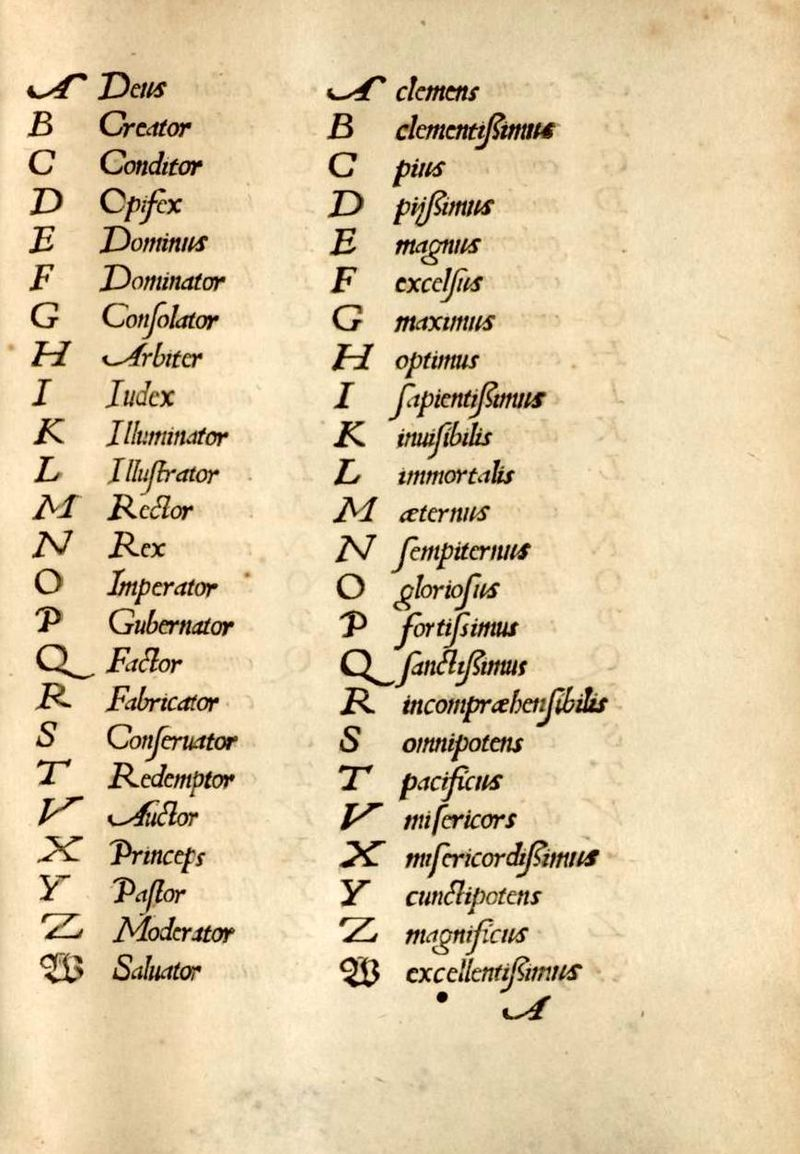
\includegraphics[scale=1.1]{images/L-Trithemius-Polygraphiae-71.jpg}
		\caption{Buchstaben-Wort-Substitutionstabelle von Buch I der Polygraphia von Johannes Trithemius, Quelle: \url{http://daten.digitale-sammlungen.de/bsb00026190/image_71}}
		\label{fig:L: Polygraphia}
	\end{figure}
	
	
	
	
	
	
	
	
	\section{Abgrenzung zur Kryptographie}
	
	Kryptographie und Steganographie werden oft gemeinsam verwendet, wodurch meist nicht genau zwischen diesen beiden Verfahren unterschieden wird. Wie man in \autoref{L: Tab: Stego VS Crypto} \todo{Wie bekommt man die richtige Bezeichnung hier in den Text(unterschied zwischen label und caption)} sehen kann, wirken beide Techniken auf den ersten Blick sehr �hnlich, sind aber bei genauerer Betrachtung zwei komplett unterschiedliche Verfahren. Wichtig ist hier vor allem zu beachten: Steganographie sch�tzt Daten nicht vor Dritten, wenn diese gezielt danach Suchen und wenn sie sich sicher sind, dass in den Informationen, die Ihnen vorliegen weitere Nachrichten versteckt wurden. Des Weiteren haben Steganogramme die Eigenschaft zwar von Menschen schlecht erkannt werden zu k�nnen, von Computern jedoch meist relativ schnell eine versteckte Nachricht sichtbar gemacht werden kann. Bei dem Erfolg eines computergest�tzten Verfahren kommt es aber sehr stark auf die verwendete Technik und die verf�gbare Rechenleistung an. 
	
	
	\begin{table}[h]
		\begin{center}
			\begin{tabular}{|l|l|}
				\hline
				\textbf{Steganographie} & \textbf{Kryptographie}\\
				\hline
				\hline
				stegano = verdeckt 	& krypte = geheim \\
				graphein = scrheiben & graphein = schreiben \\
				\hline
				Die Nachricht wird verborgen, & Die Nachricht wird verschl�sselt \\
				nicht verschl�sselt & nicht verborgen \\
				\hline
				Scheinbar existiert gar & Die Nachricht existiert, kann aber\\
				keine Nachricht & nicht gelesen werden \\
				\hline
			\end{tabular}
		\end{center}
		\caption{Vergleich zwischen Steganographie und Kryptographie, Quelle: \cite{L: Stego VS Crypto}} 
		\label{L: Tab: Stego VS Crypto}
	\end{table}
	
	Am sichersten ist es, wenn man beide Verfahren kombiniert. Dadurch hat man nicht nur die Vorteile der Kryptographie (Vertraulichkeit, Integrit�t und Authentizit�t), sondern auch die der Steganographie. Interessant ist hier vor allem die Eigenschaft von Verschl�sselungen: Diese gelten dann als sicher, wenn sie den Klartext derart ver�ndern, dass er keine statistischen Merkmale des urspr�nglichen Text mehr aufweist. 
	Der Geheimtext kann also bei guten Verschl�sselungsverfahren statistisch nicht mehr von Rauschen unterschieden werden. Wenn man dieses ''Rauschen'' dann mit Hilfe von Steganographie in ein unauff�lliges Tr�germedium einbettet, ist es selbst mit elektronischer Datenverarbeitung nicht mehr m�glich, eine Nachricht im Steganogramm zu entdecken. Die einzige M�glichkeit f�r Dritte hier noch etwas herauszufinden, ist es das Steganogramm mit dem originalen Tr�germaterial zu vergleichen. Hier fallen dann Unterschiede auf. Diese Technik ist aber in der Praxis selten anwendbar, denn einzigartige Tr�germaterialien k�nnen sehr leicht hergestellt werden (\zb Digitalfotografie) und weil das Tr�germedium nicht zum Dekodieren ben�tigt wird, kann das Original nach der Erstellung des Steganogramm gel�scht werden.
	
	
	
	\section{Einsatzgebiete}
	
	Steganographie sch�tzt Daten nicht vor Missbrauch, warum sollte man sie dann �berhaupt verwenden, wenn Kryptographie viel sicherer ist? In der westlichen Welt ist Verschl�sselung durch das Internet so weit verbreitet, dass es als selbstverst�ndlich erscheint, seine Daten und Konversationen verschl�sselt zu speichern. Doch in vielen L�ndern ist es auch heute noch illegal solche Techniken einzusetzen. Selbst in den Vereinigten Staaten von Amerika gab es noch bis in das Jahr 2000 sehr   restriktive Gesetze was Verschl�sselung anbelangt. Das f�hrte soweit, dass sogar ein T-Shirt auf welches der Source-Code f�r RSA-Encryption gedruckt wurde, unter das Waffengesetz fiel, als ''export-restricted munition'' deklariert und f�r den Export verboten wurde.
	
	Hier kommt Steganographie zum Einsatz. Sie bietet eine M�glichkeit seine Daten und sich selber trotz der lokal geltenden Gesetze zu sch�tzen. Nicht nur dass es schwer zu erkennen ist, ob sich �berhaupt versteckte Daten auf einem Laufwerk befinden, steganographische Verfahren werden meist gar nicht von den Gesetzten verboten. Man befindet sich meist in einer Grauzone, was einem einen gewissen Verhandlungsspielraum verschafft. 
	
	Sie bietet auch Schutz vor potentiellen Hackern. Denn w�hrend bei verschl�sselten Daten ein sich lohnendes Ziel auf den Angreifer wartet, ist es bei Steganographie sehr unwahrscheinlich etwas Verwertbares zu finden, falls �berhaupt etwas vorhanden ist. Dadurch macht man sich als Opfer sehr unattraktiv.
	
	\cite{L: StegoVersteck}
	
	\section{Steganographie als ''Wicked Problem''}
	
	Die Steganographie besitzt viele Eigenschaften von sogenannten ''Wicked Problems''. 
	
	\begin{itemize}
		\item Es gibt keine genaue Definition des Problems
		\item Sie haben keine Stopp-Regel (''Hat man auch wirklich nichts �bersehen?'')
		\item Es gibt keinen ultimativen und sofortigen Test f�r die Richtigkeit von L�sungen des Problems
		\item Wicked Problems haben weder eine abz�hlbare L�sungsmenge, noch gibt es eine gut beschriebene Gruppe an g�ltigen Operatoren
	\end{itemize}
	
	Diese Eigenschaften und die Tatsache das Kommunikation schwer zu definieren ist, f�hren dazu, dass paranoide oder phantasievolle Menschen glauben, Nachrichten zu empfangen, obwohl keine vorhanden sind. Da k�nnen selbst kleine unbedeutende Handlungen von Mitmenschen als geheime Nachrichten�bertragung interpretiert werden, was unter anderem zu Problemen f�hren kann, wo eigentlich keine sind. 
	
	Doch auch in der Verbrechensaufkl�rung kann die Wicked-Problem Eigenschaft von Steganographie zum Problem werden. Wird hier denn wirklich neben der offensichtlich �bertragenen Information noch eine versteckte Nachricht mitgesendet? Eine verd�chtige Person kauft jeden Tag einen Kaffee auf dem Weg zur Arbeit. Die Verk�uferin ist die Freundin von dem Steuerberater des Chefs des Verd�chtigen. Pl�tzlich kauft er aber einen Kr�utertee. Hat er jetzt den Steuerberater vor irgendetwas gewarnt oder hat er heute nur Halsweh und m�chte seinen Hals schonen? Das ist eben die Natur von Wicked Problems. Man kann sich nie sicher sein, denn es gibt weder eine genaue Fragestellung, noch ein eindeutiges Erfolgskriterium oder eine klar definierte Ausgangslage. 
	
	
	
	
	
	
	
	
	\clearpage
	
%--------------------------------------------------------------------------
% Anhang
%--------------------------------------------------------------------------

  \phantomsection
  \addcontentsline{toc}{chapter}{Anhang}
	\addcontentsline{toc1}{section}{Abbildungsverzeichnis}
	\listoffigures
	\newpage
	\phantomsection
	
	\addcontentsline{toc}{section}{Tabellenverzeichnis}
	\listoftables
	\newpage
	\phantomsection

	\addcontentsline{toc}{section}{Verzeichnis der Listings}
	\lstlistoflistings
	\newpage
	\phantomsection
	
	%\addcontentsline{toc}{section}{Index}
  \printindex
  \newpage
  \phantomsection
  
	\addcontentsline{toc}{section}{Literaturverzeichnis}
	%\bibliographystyle{alpha} 		 %Standardstyle
	%\bibliographystyle{dinat}		 %Style und Layout nach DIN 1502
	%\bibliography{tiger}					 %Literaturverzeichnis einf�gen
	
	
	%So kann zitiert werden (sollte in einer der Unterdateien sein)
	%\citep[vgl. Seite 22]{kopka1:00}
	
	\begin{thebibliography}{999}
		

\bibitem[S: StegoGeschichte]{S: StegoGeschichte} 
\href{https://igw.tuwien.ac.at/designlehren/steganographie.pdf}{https://igw.tuwien.ac.at/designlehren/steganographie.pdf} \\
Eine kurze Geschichte der Steganographie \\ 
Peter Purgathofer \\
12.11.2016
		
		\bibitem[Kopka1]{kopka1:00} 
		Helmut Kopka:
		  \emph{Latex Band 1, Einf�hrung} \\ 
		  Addison-Wesley, 2000  \\
		  ISBN: 3-8273-7038-8
		\bibitem[Demmig 1]{demig:04}
		  Demmig, Thomas: \\
			\emph{jetzt lerne ich Latex 2} \\
			Markt+Technik, 2004 \\
			ISBN 3-8272-6517-7
		\bibitem[Web 1]{Web:01}
		\href{http://www.meta-x.de/faq/LaTeX-Einfuehrung.html}{http://www.meta-x.de/faq/LaTeX-Einfuehrung.html}\\
		Latex-Einf"uhrung\\
		28.September 2012
		\bibitem[JavaDoc05]{JavaDoc:05}
		\href{http://docs.oracle.com/cd/E12839\_01/core.1111/e10043/introjps.htm}{http://docs.oracle.com/cd/E12839\_01/core.1111/e10043/introjps.htm}\\
		Oracle Security Guide �ber das Java Sicherheits Model\\
		13.11.2014
	\end{thebibliography} 
	\newpage
	\phantomsection
\end{document}